\documentclass[tikz]{standalone}
\usetikzlibrary{patterns}
\begin{document}
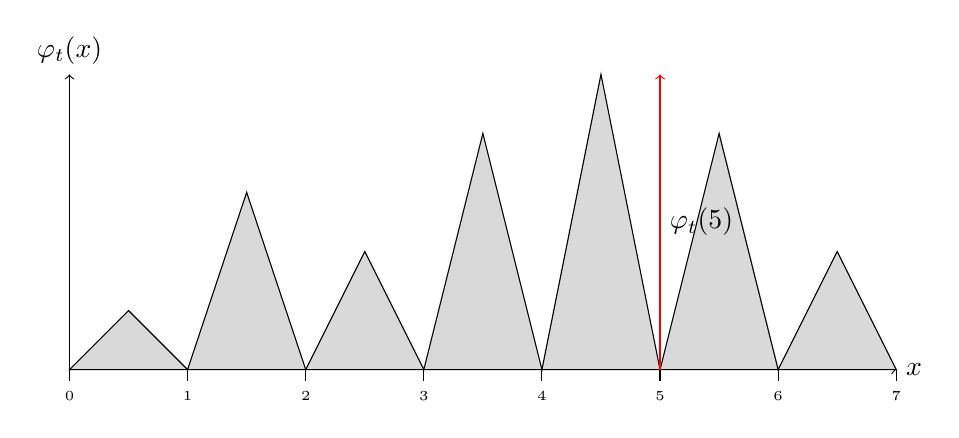
\begin{tikzpicture}[xscale=1.5, yscale=1.5]
  % Draw the x-axis
  \draw[->] (0,0) -- (7,0) node[right] {$x$};
  \draw[->] (0,0) -- (0,2.5) node[above] {$\varphi_t(x)$};
  
  % Draw the fluctuating interface
  \draw[fill=gray!30] 
    (0,0) -- (0.5,0.5) -- (1,0) -- (1.5,1.5) -- (2,0) 
    -- (2.5,1) -- (3,0) -- (3.5,2) -- (4,0) -- (4.5,2.5) 
    -- (5,0) -- (5.5,2) -- (6,0) -- (6.5,1) -- (7,0) -- cycle;
  
  % Highlight the peak at x=5 with a red arrow
  \draw[red,->] (5,0) -- (5,2.5) node[midway, right, black] {$\varphi_t(5)$};
  
  % Mark the lattice points
  \foreach \x in {0,1,...,7} {
    \draw (\x,0) -- (\x,-0.1) node[below] {\tiny$\x$};
  }
\end{tikzpicture}
\end{document}